%! TEX root = ../main.tex
\documentclass[main]{subfiles}

\begin{document}

\section{表面の繊維}

まず,一番ゴミが付着しているカーリングブラシパッドの縁の部分の写真は以下のとおりである.

\begin{itemize}
    \item 未使用×1
    \begin{figure}[H]
        \centering
        \begin{minipage}[htbp]{0.45\linewidth}
            \centering
            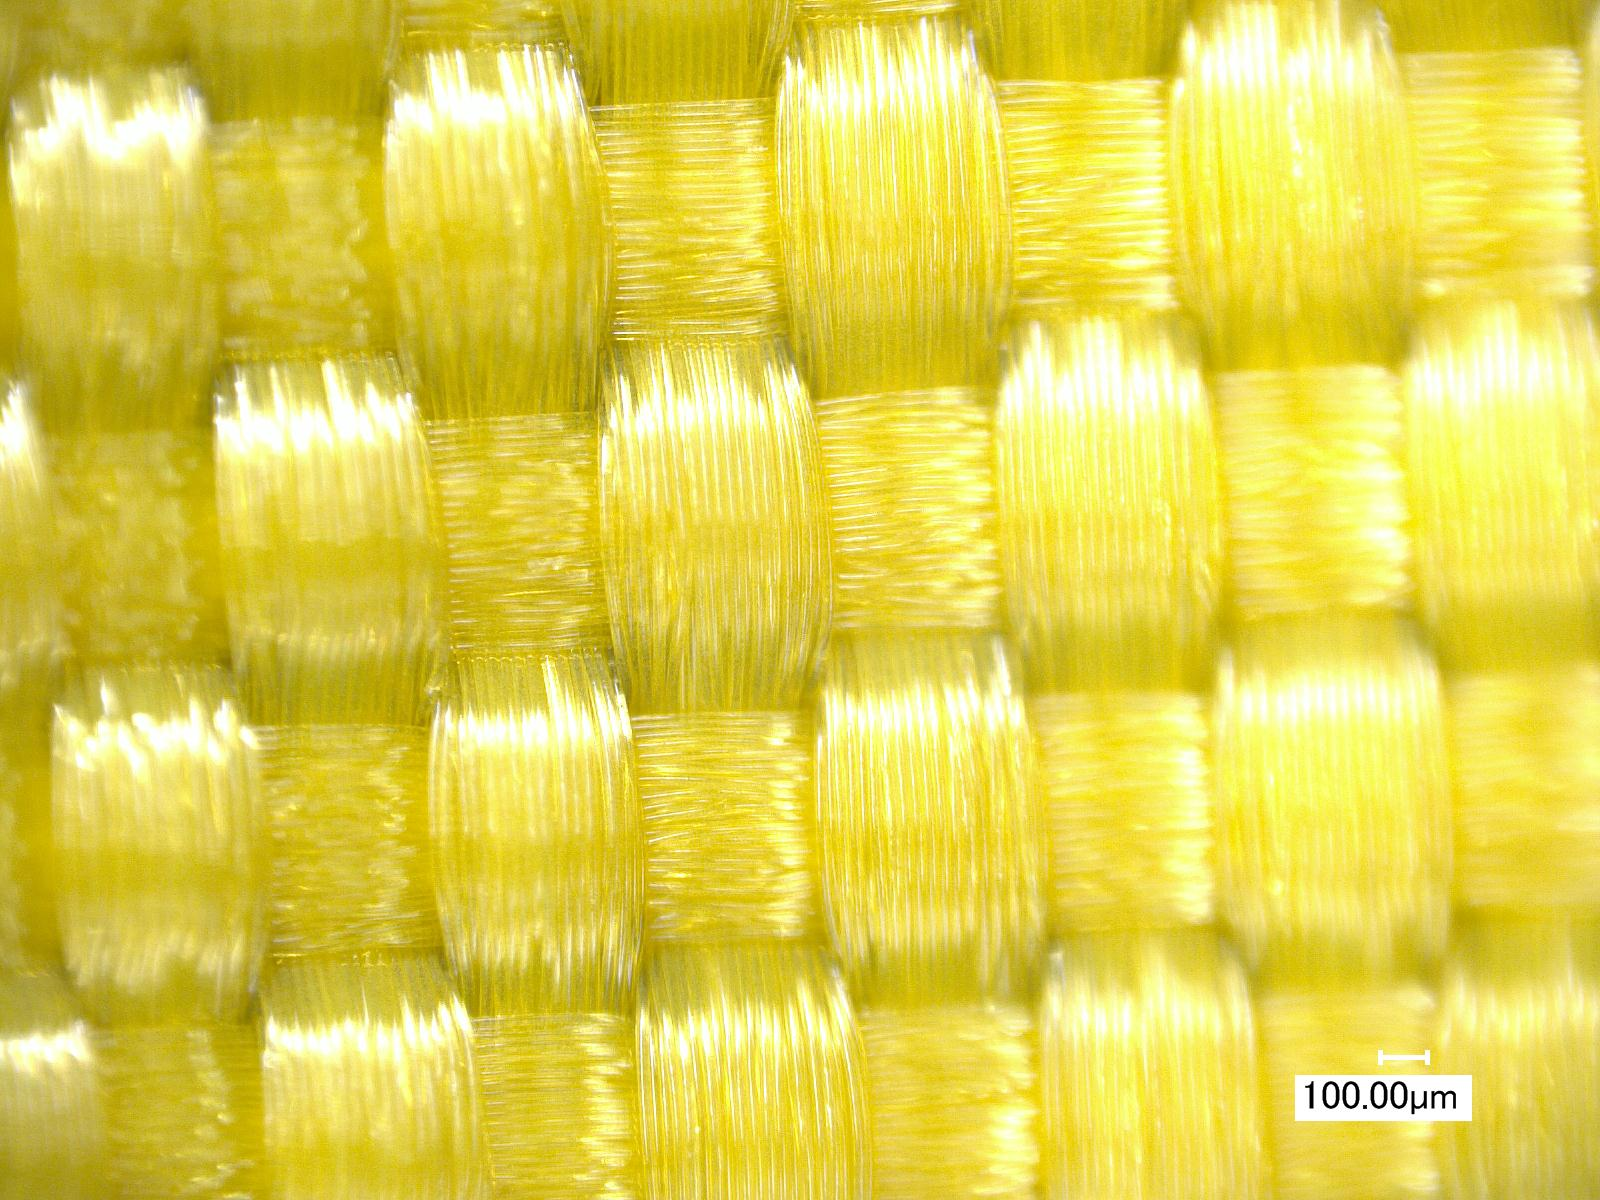
\includegraphics[keepaspectratio, width=0.8\linewidth]{figures/縁/カーリングパッド未使用低倍率.jpg}
            \caption{低倍率(100倍)}
            \label{fig:label}
        \end{minipage}
        \begin{minipage}[htbp]{0.45\linewidth}
            \centering
            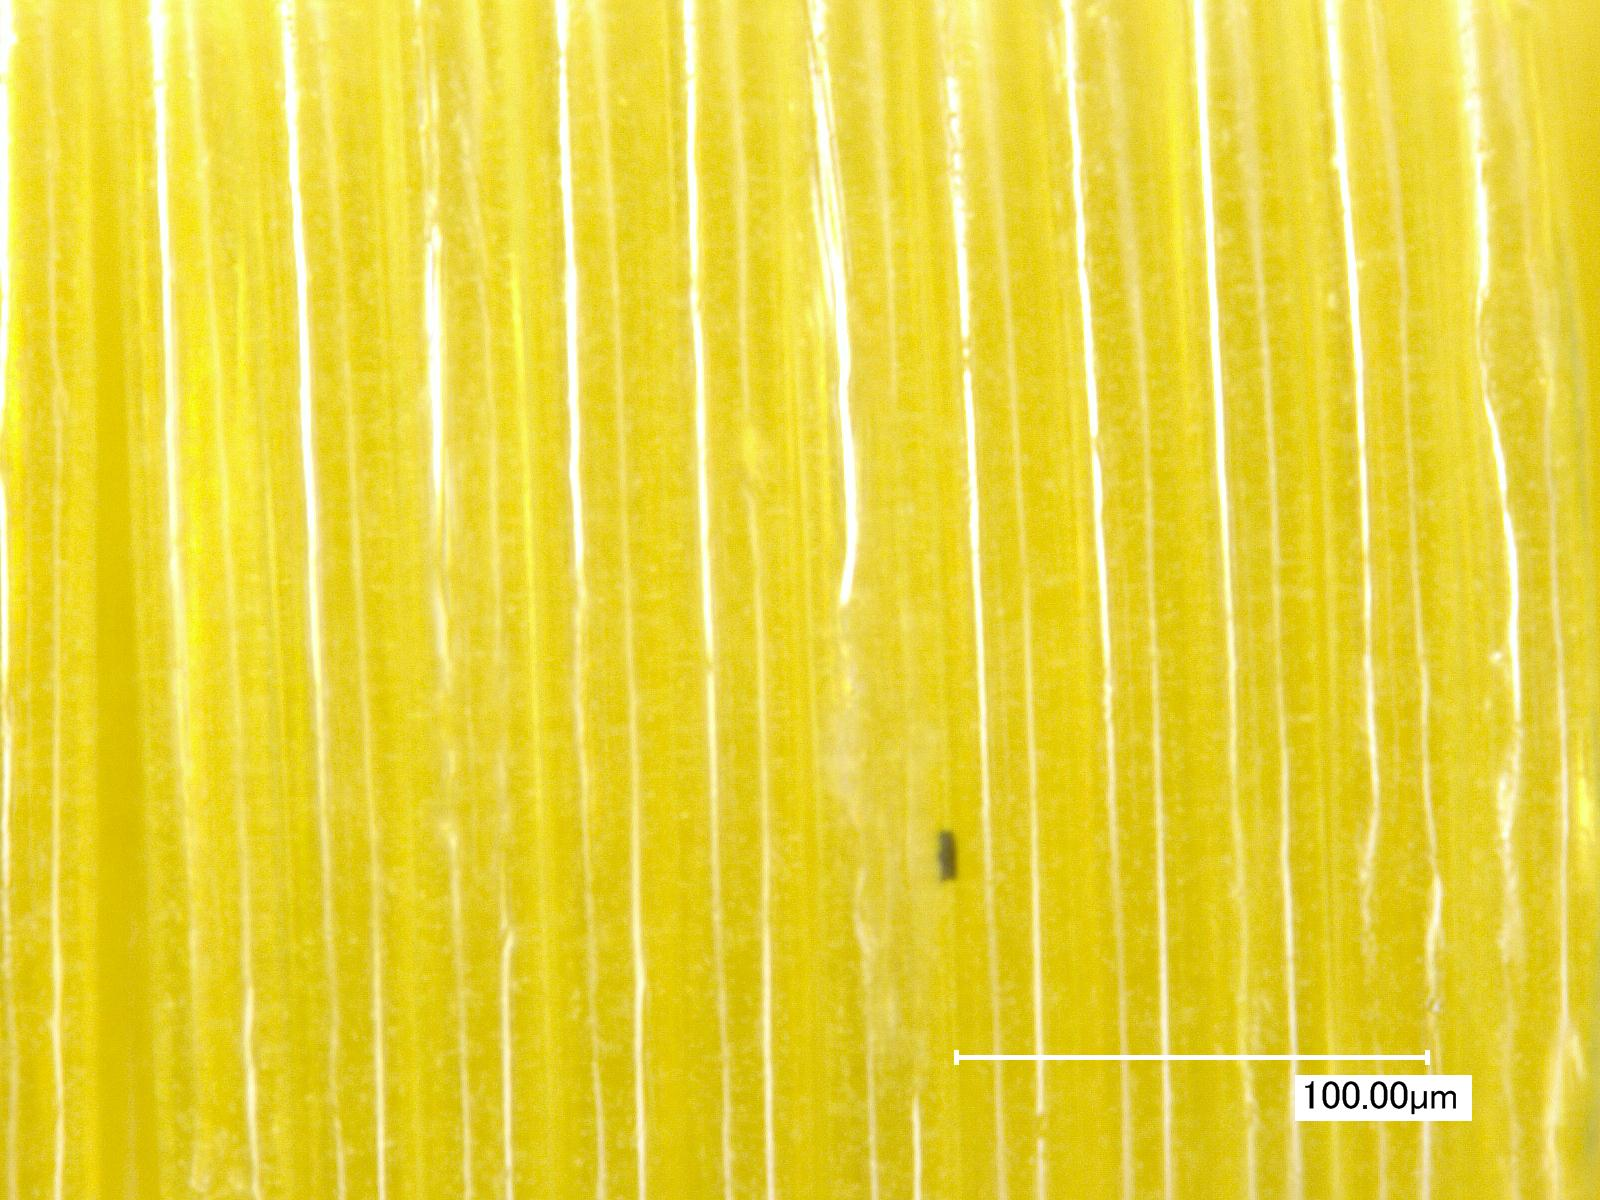
\includegraphics[keepaspectratio, width=0.8\linewidth]{figures/縁/カーリングパッド未使用.jpg}
            \caption{高倍率(1000倍)}
            \label{fig:label}
        \end{minipage}
    \end{figure}
    
    \item 10~15投使用×2
    サンプルA
    \begin{figure}[H]
        \centering
        \begin{minipage}[htbp]{0.45\linewidth}
            \centering
            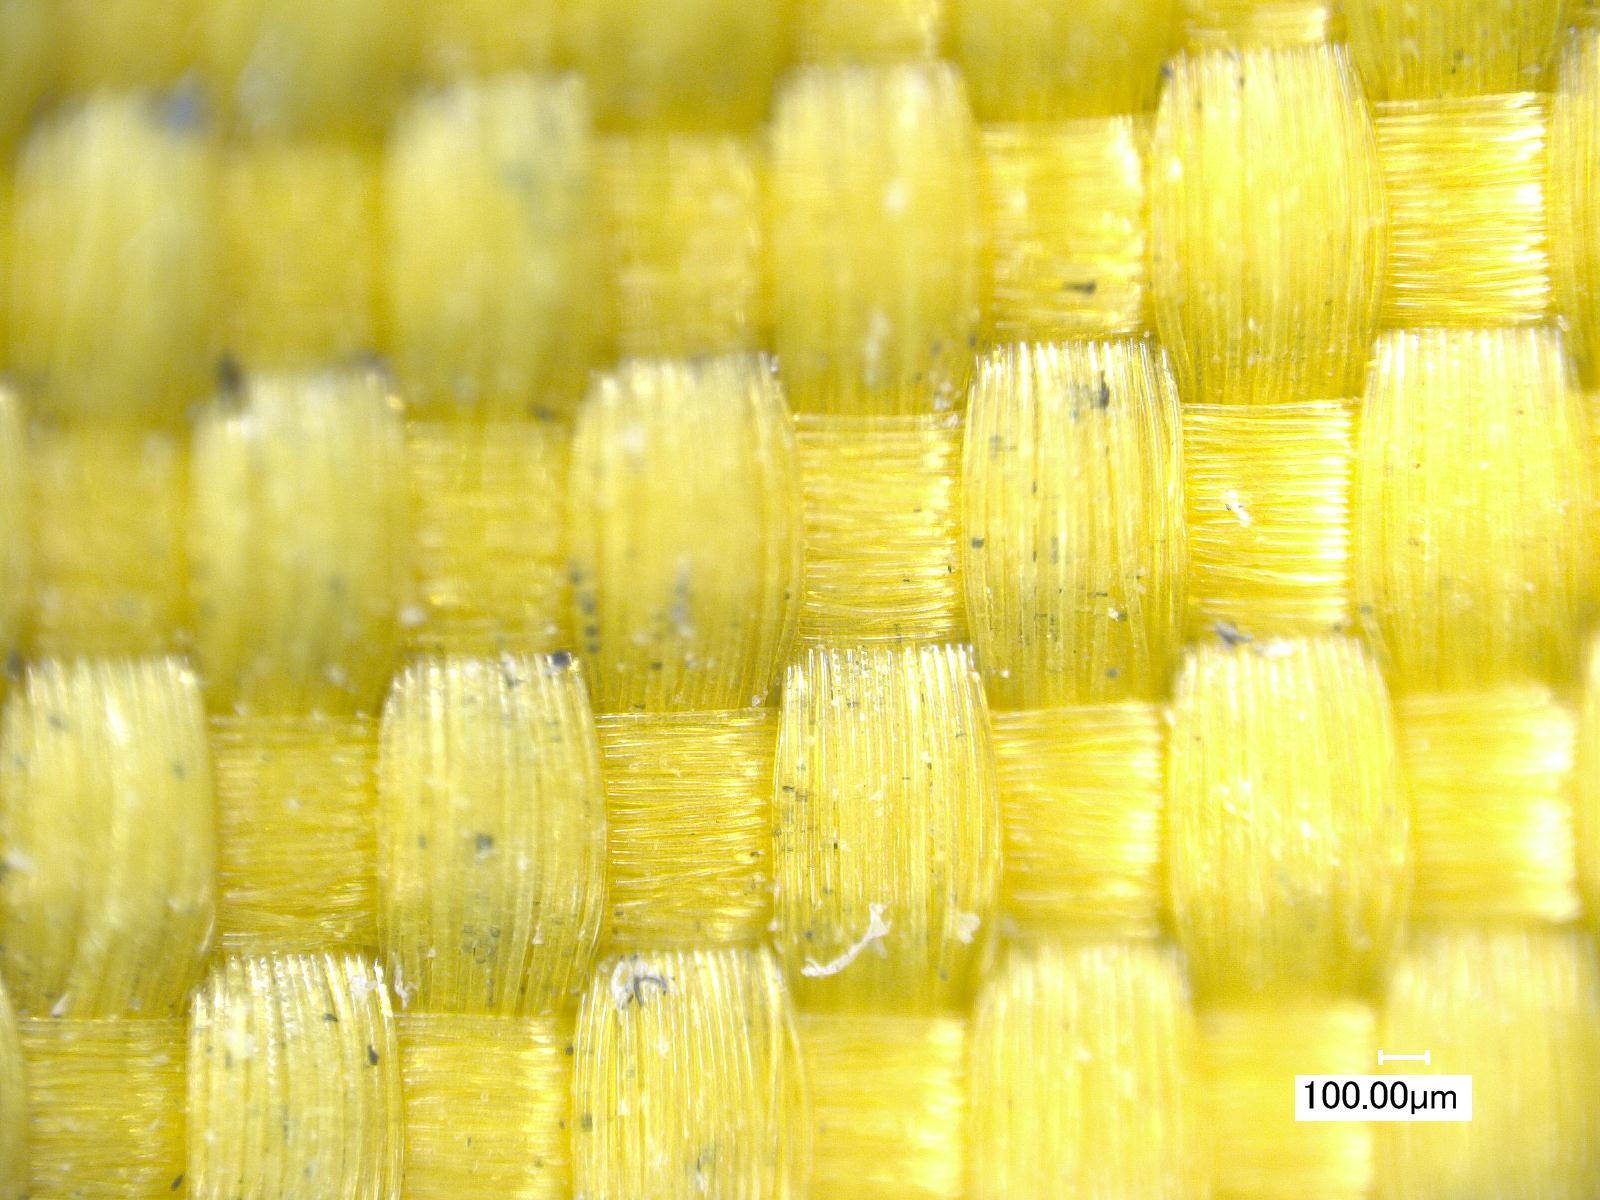
\includegraphics[keepaspectratio, width=0.8\linewidth]{figures/縁/カーリングパッド10-15低倍率.jpg}
            \caption{低倍率(100倍)}
            \label{fig:label}
        \end{minipage}
        \begin{minipage}[htbp]{0.45\linewidth}
            \centering
            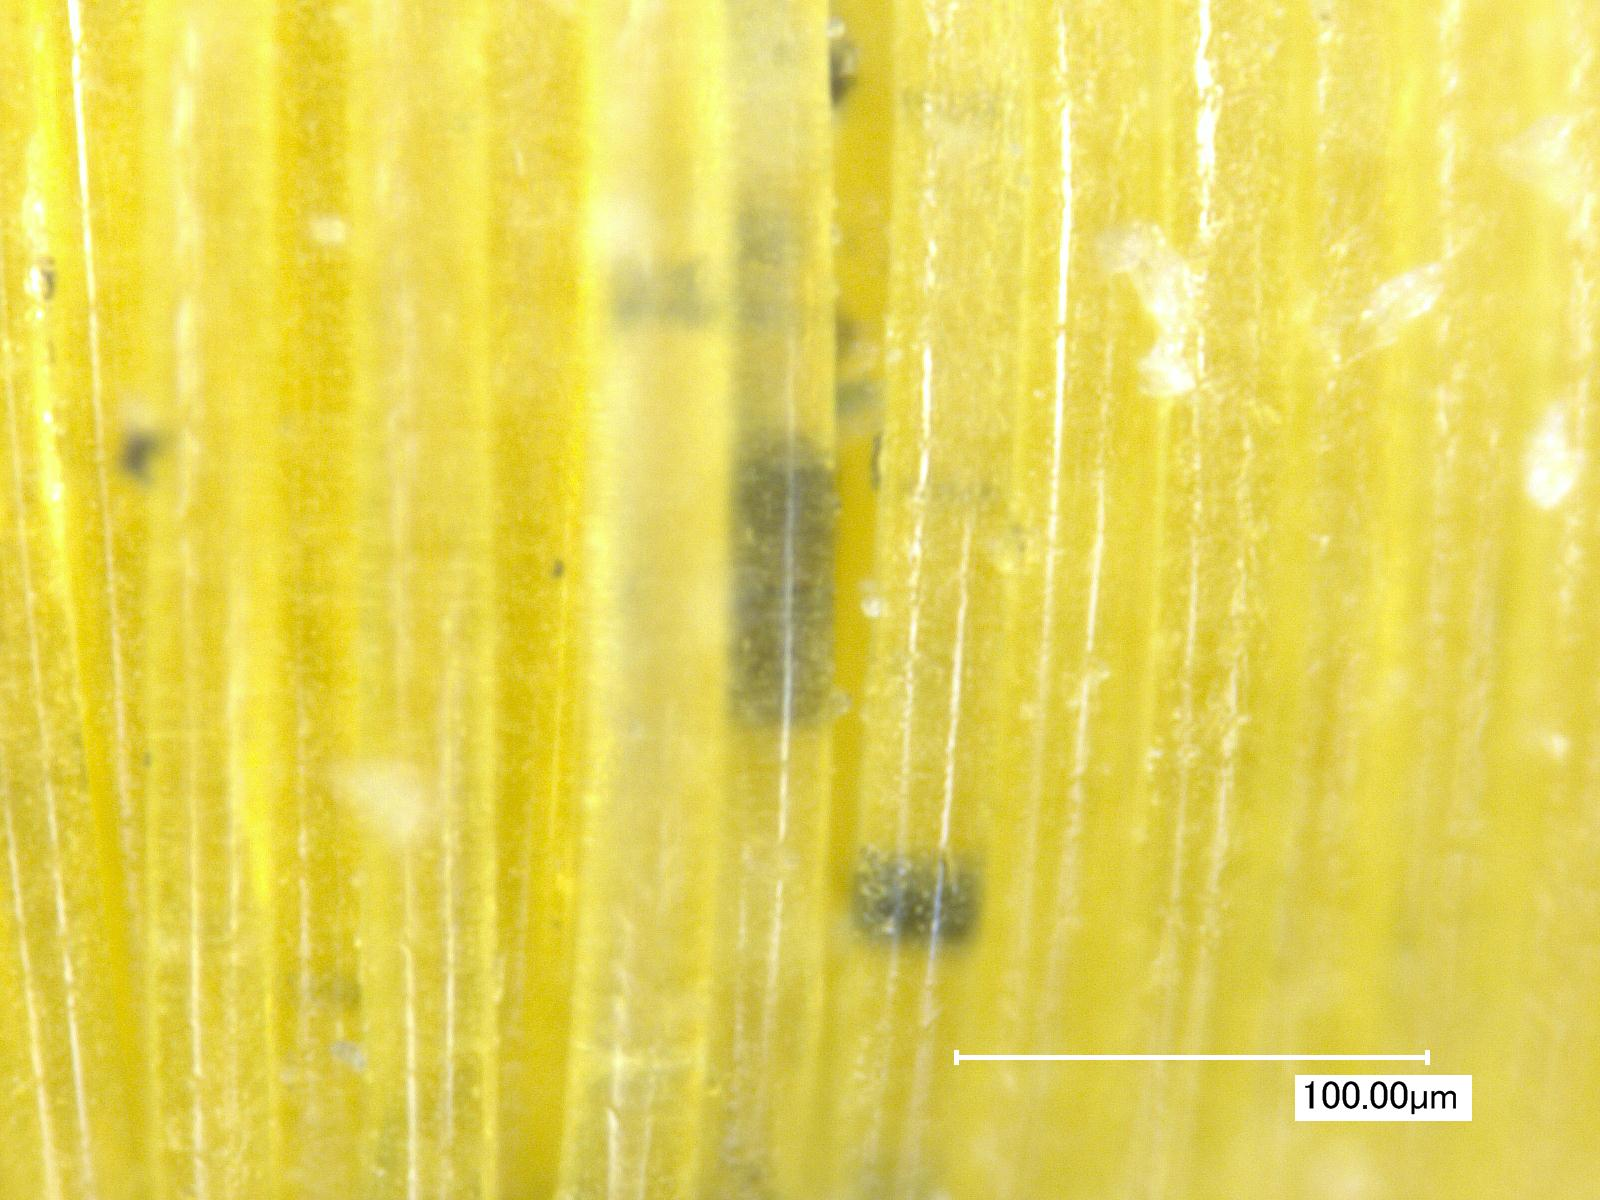
\includegraphics[keepaspectratio, width=0.8\linewidth]{figures/縁/カーリングパッド10-15.jpg}
            \caption{高倍率(1000倍)}
            \label{fig:label}
        \end{minipage}
    \end{figure}
    
    サンプルB
    \begin{figure}[H]
        \centering
        \begin{minipage}[htbp]{0.45\linewidth}
            \centering
            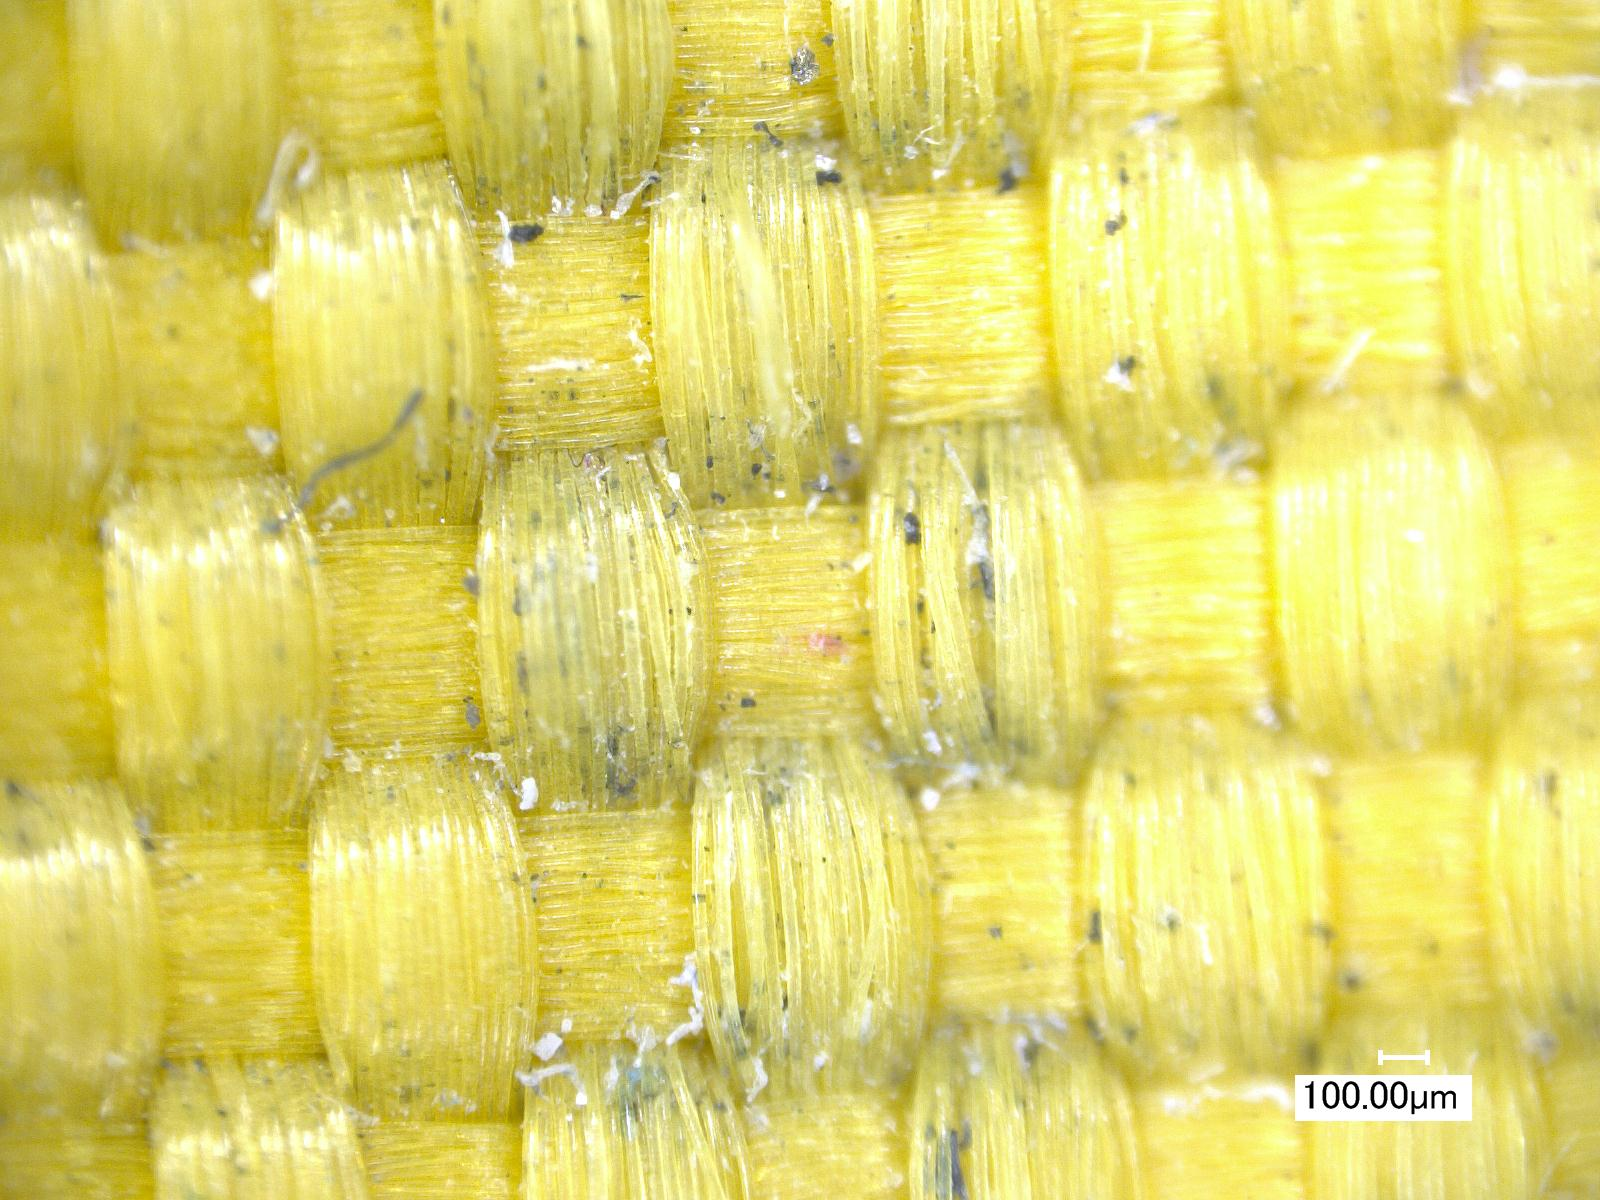
\includegraphics[keepaspectratio, width=0.8\linewidth]{figures/縁/カーリングパッド10-15低倍率B.jpg}
            \caption{低倍率(100倍)}
            \label{fig:label}
        \end{minipage}
        \begin{minipage}[htbp]{0.45\linewidth}
            \centering
            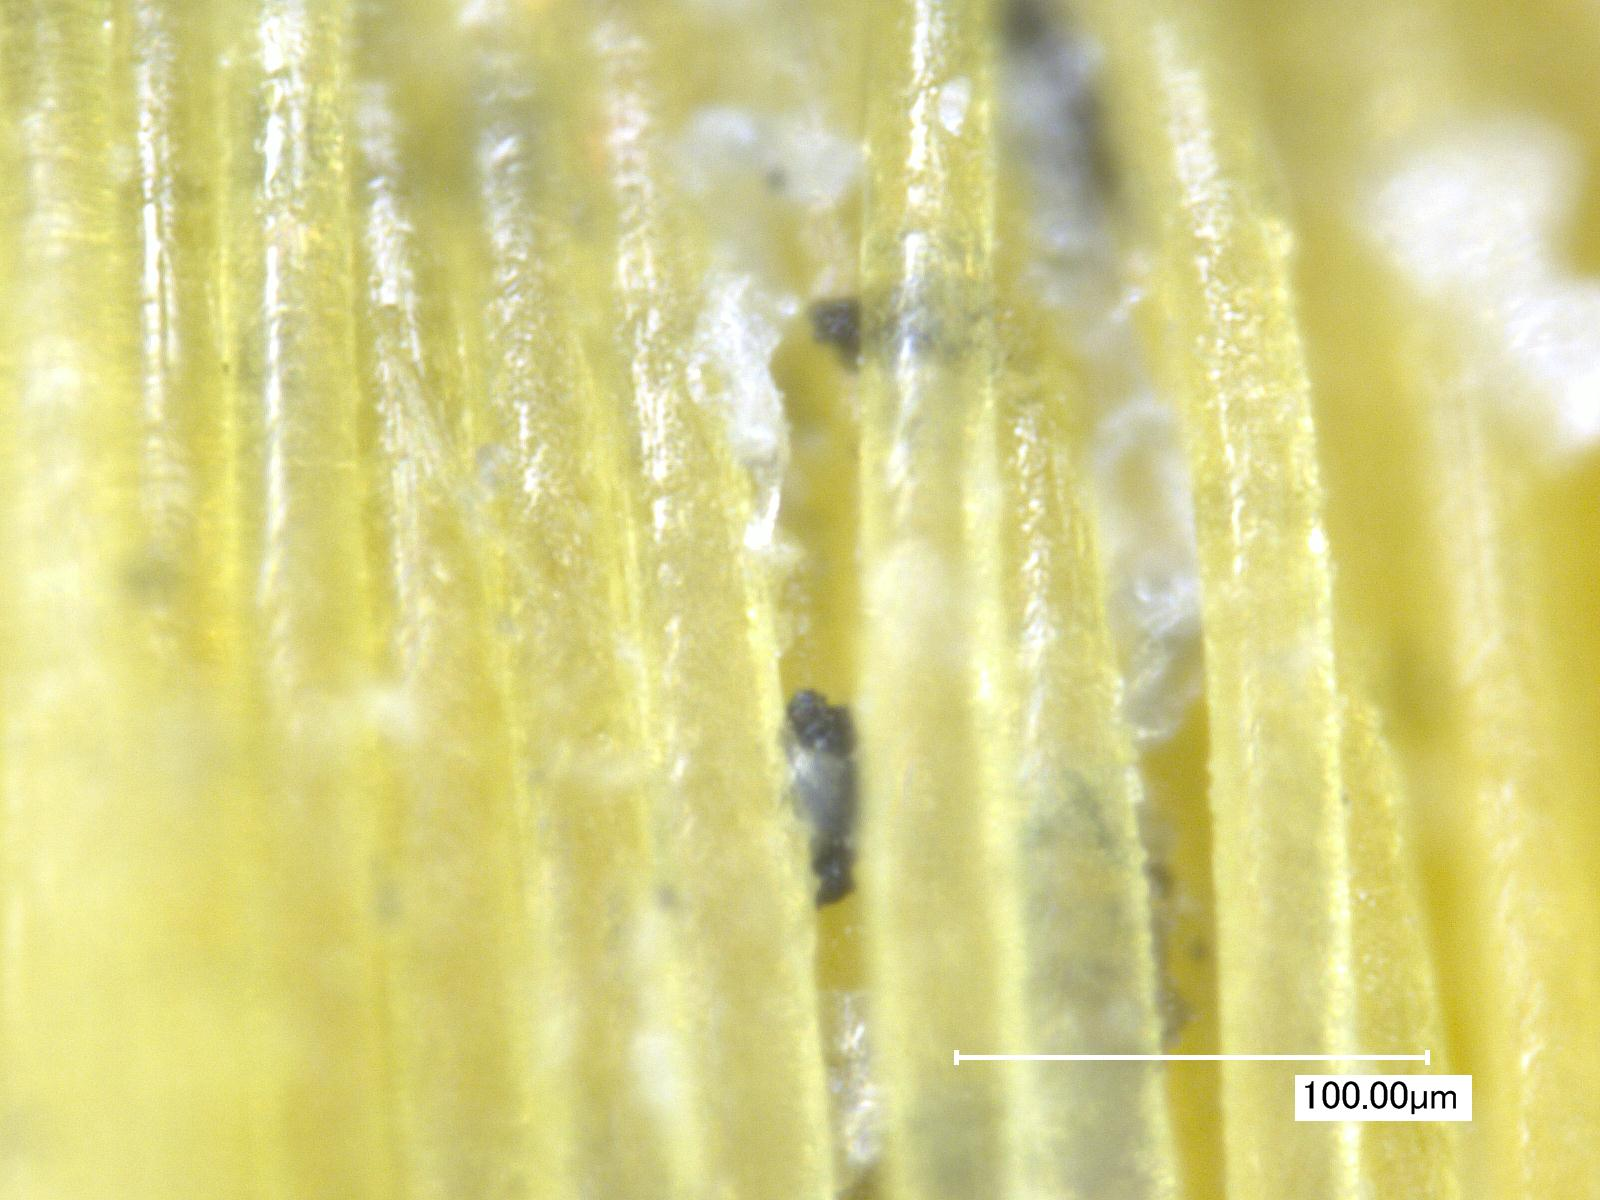
\includegraphics[keepaspectratio, width=0.8\linewidth]{figures/縁/カーリングパッド10-15B.jpg}
            \caption{高倍率(1000倍)}
            \label{fig:label}
        \end{minipage}
    \end{figure}

    \item 長時間使用×2
    サンプルA
    \begin{figure}[H]
        \centering
        \begin{minipage}[htbp]{0.45\linewidth}
            \centering
            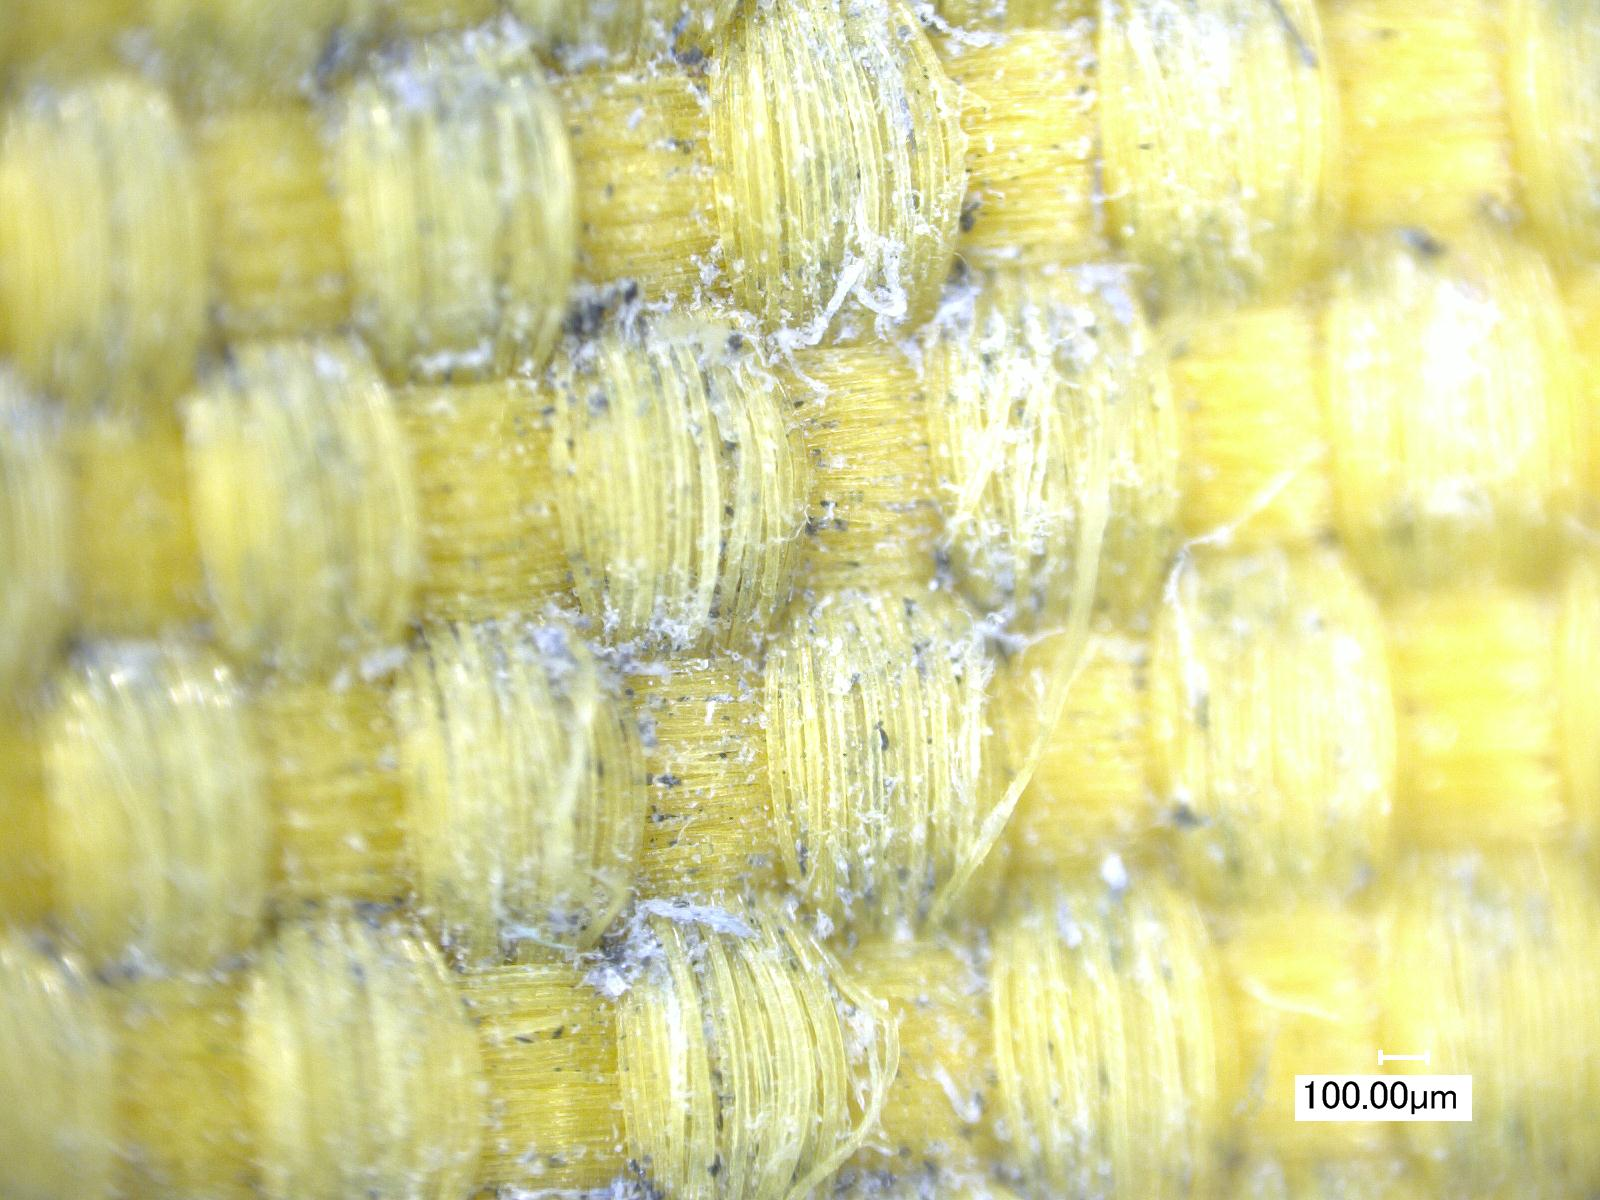
\includegraphics[keepaspectratio, width=0.8\linewidth]{figures/縁/カーリングパッド長期低倍率.jpg}
            \caption{低倍率(100倍)}
            \label{fig:label}
        \end{minipage}
        \begin{minipage}[htbp]{0.45\linewidth}
            \centering
            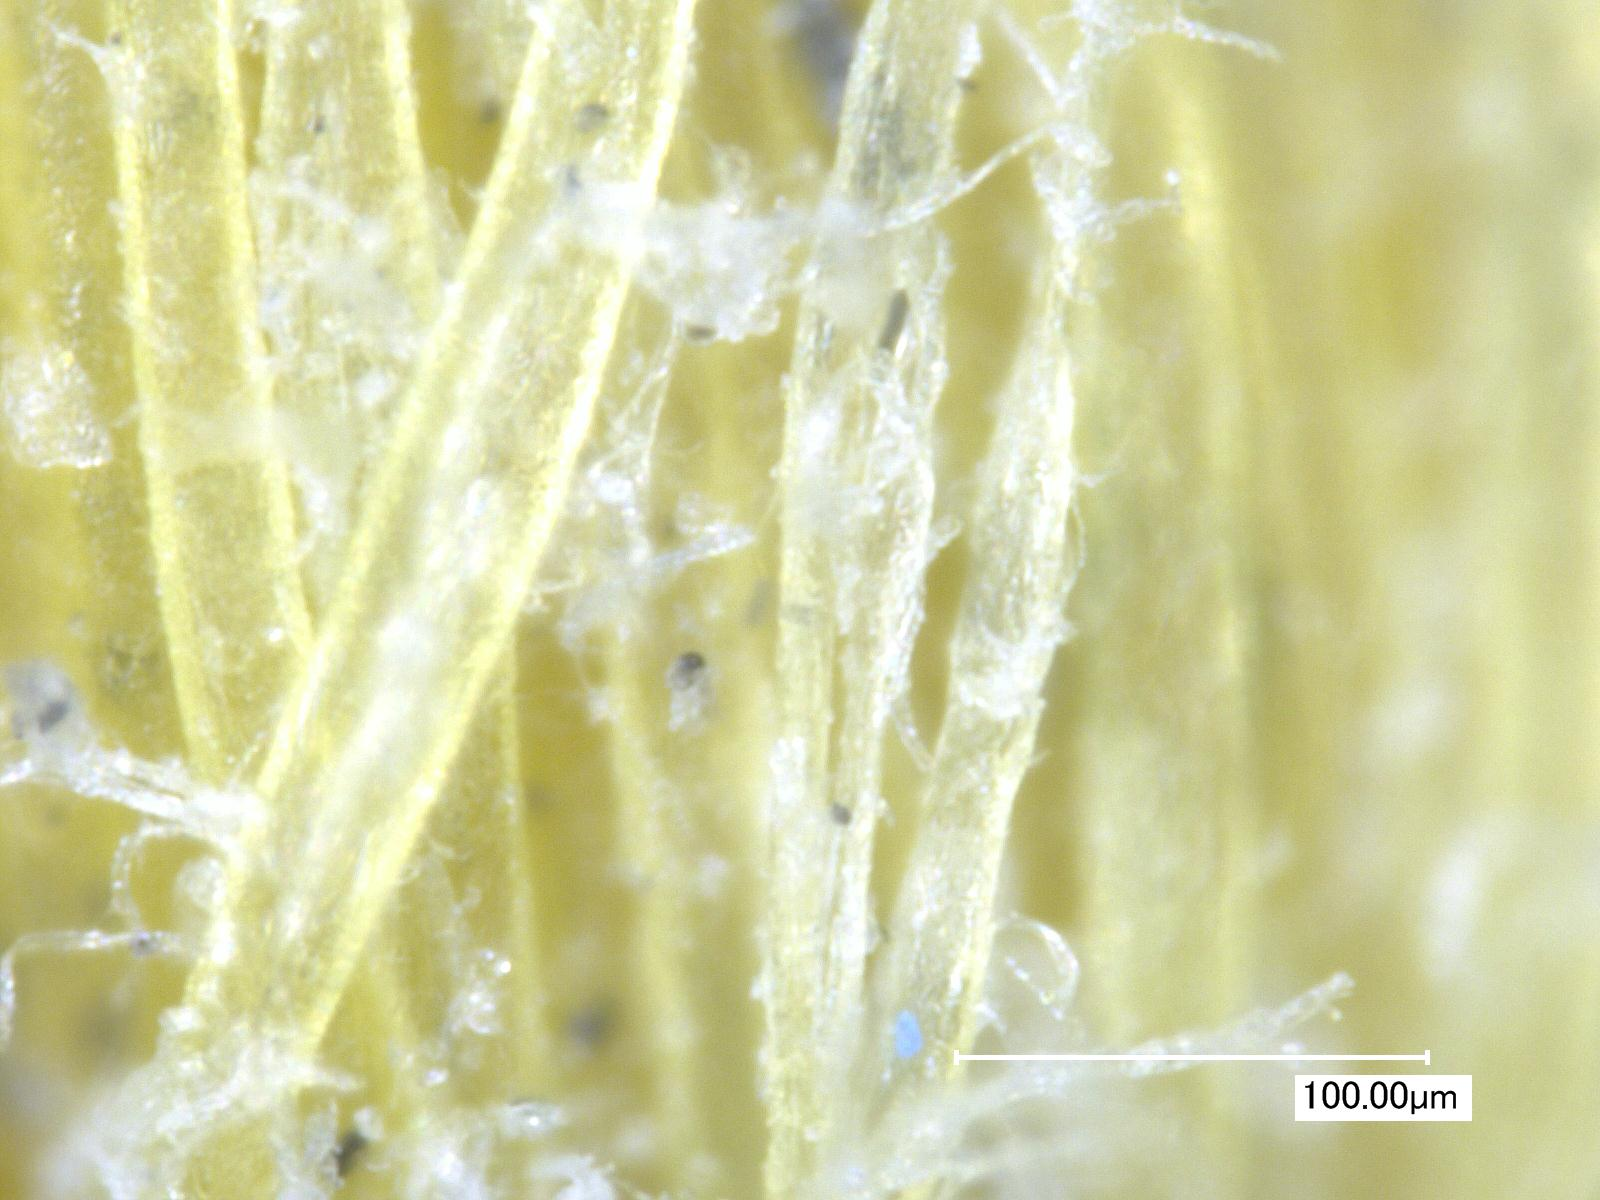
\includegraphics[keepaspectratio, width=0.8\linewidth]{figures/縁/カーリングパッド長期.jpg}
            \caption{高倍率(1000倍)}
            \label{fig:label}
        \end{minipage}
    \end{figure}
    
    サンプルB
    \begin{figure}[H]
        \centering
        \begin{minipage}[htbp]{0.45\linewidth}
            \centering
            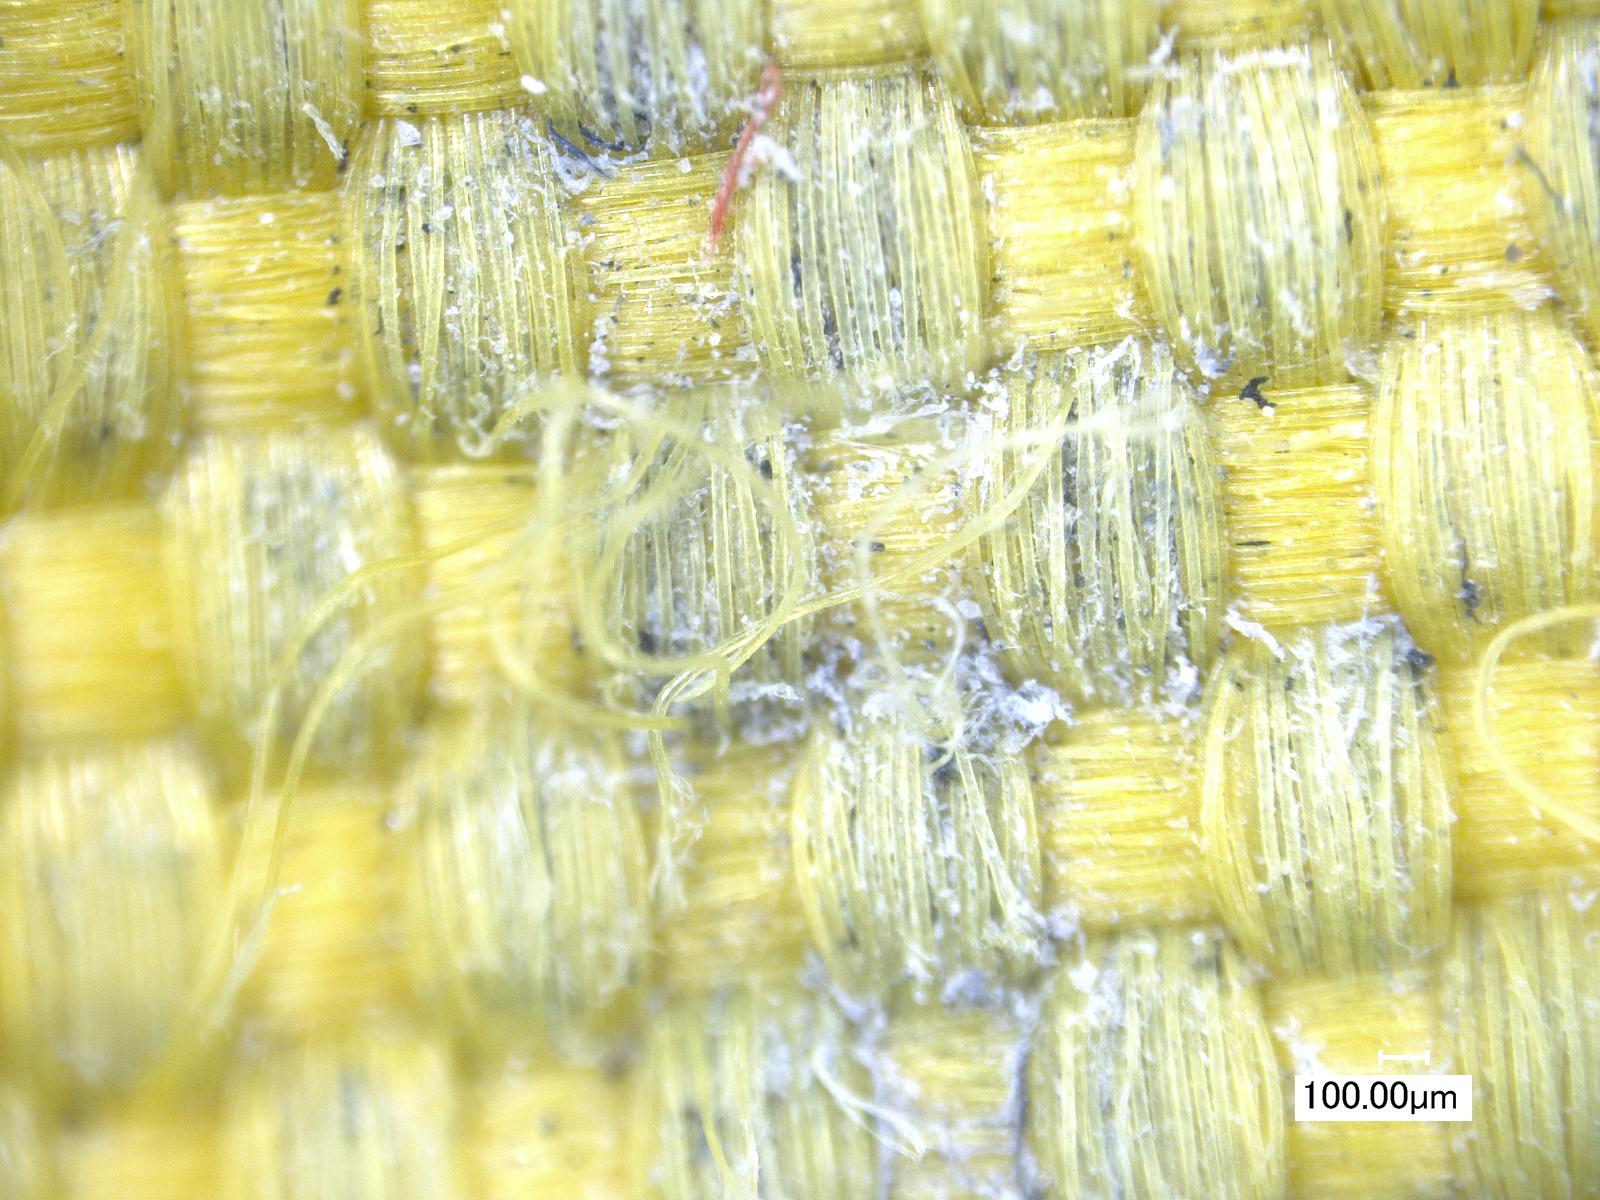
\includegraphics[keepaspectratio, width=0.8\linewidth]{figures/縁/カーリングパッド長期低倍率B.jpg}
            \caption{低倍率(100倍)}
            \label{fig:label}
        \end{minipage}
        \begin{minipage}[htbp]{0.45\linewidth}
            \centering
            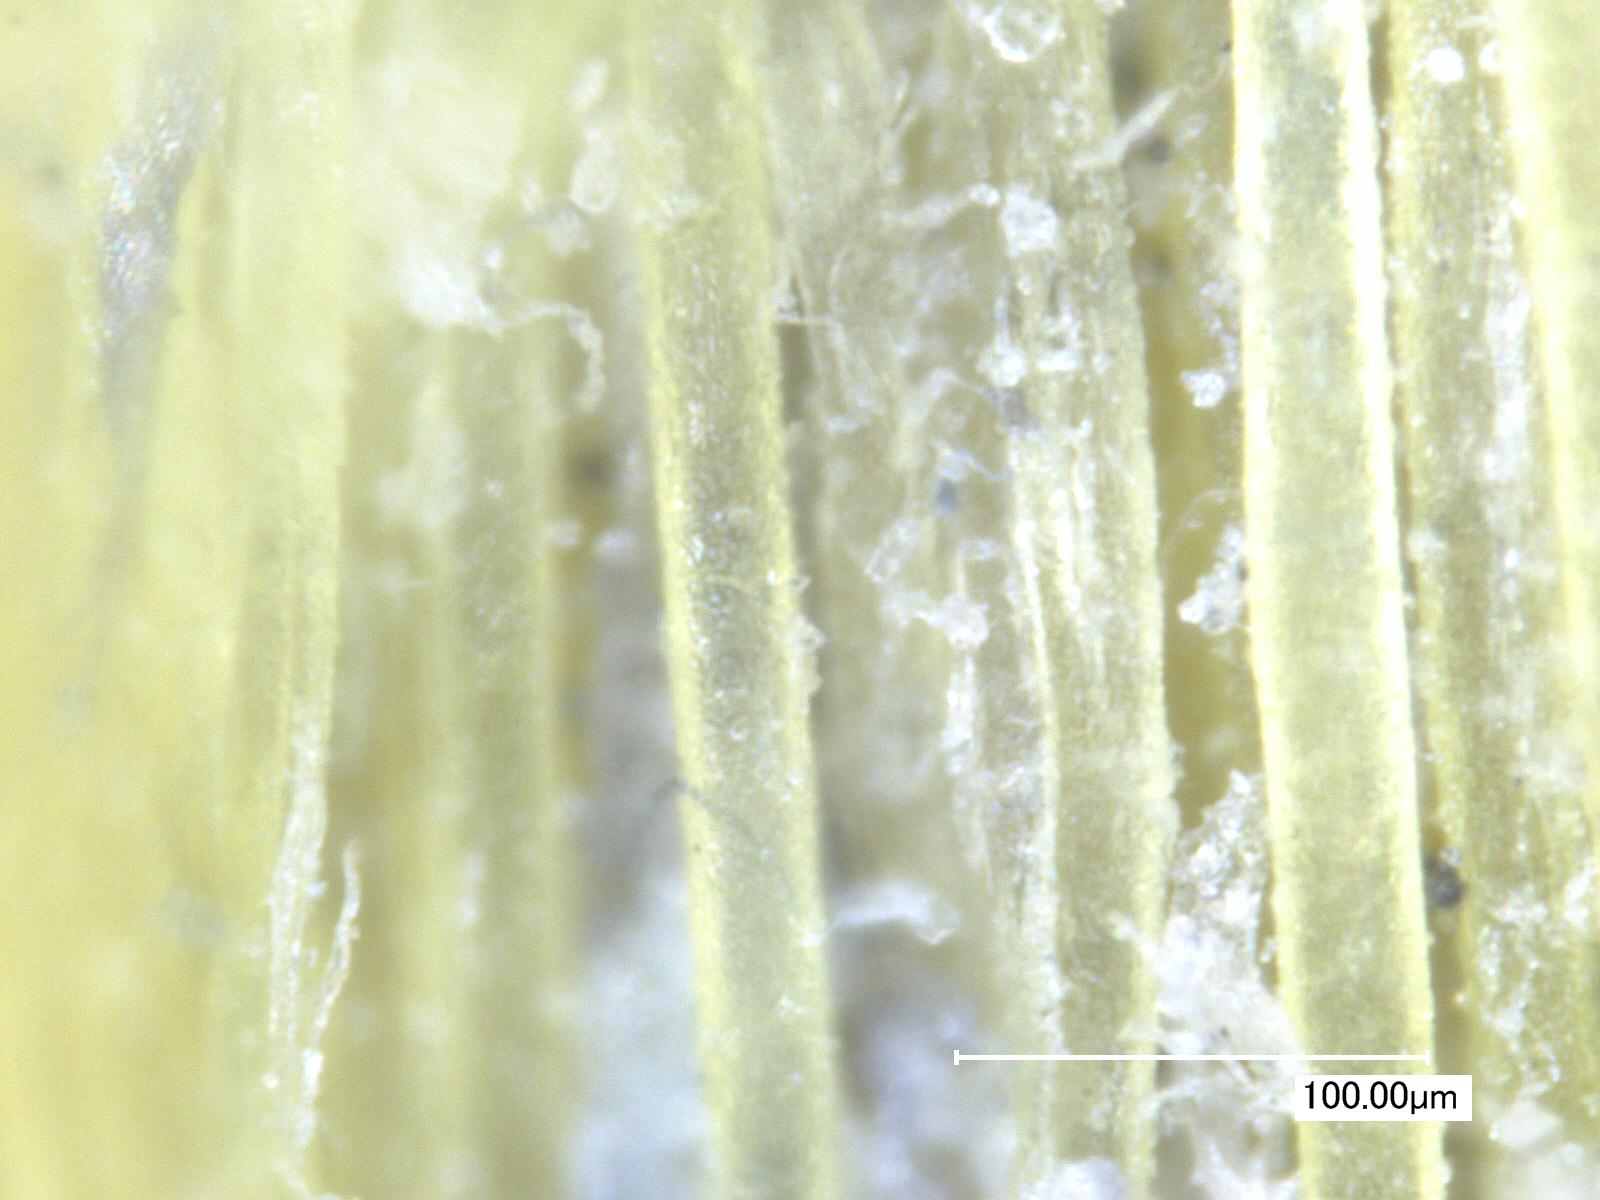
\includegraphics[keepaspectratio, width=0.8\linewidth]{figures/縁/カーリングパッド長期B.jpg}
            \caption{高倍率(1000倍)}
            \label{fig:label}
        \end{minipage}
    \end{figure}
\end{itemize}

未使用のものは1本1本の繊維が隙間なく並んでいるのに対して,10~15投使用したものは隙間が増え,長期間使用
したものは繊維が切れているものもある.
10~15投使用したものは2つのサンプルで摩耗具合が違った.

次に中心の部分の結果は以下の通りになった.

\begin{itemize}
    \item 10~15投使用
    \begin{figure}[H]
        \centering
        \begin{minipage}[htbp]{0.45\linewidth}
            \centering
            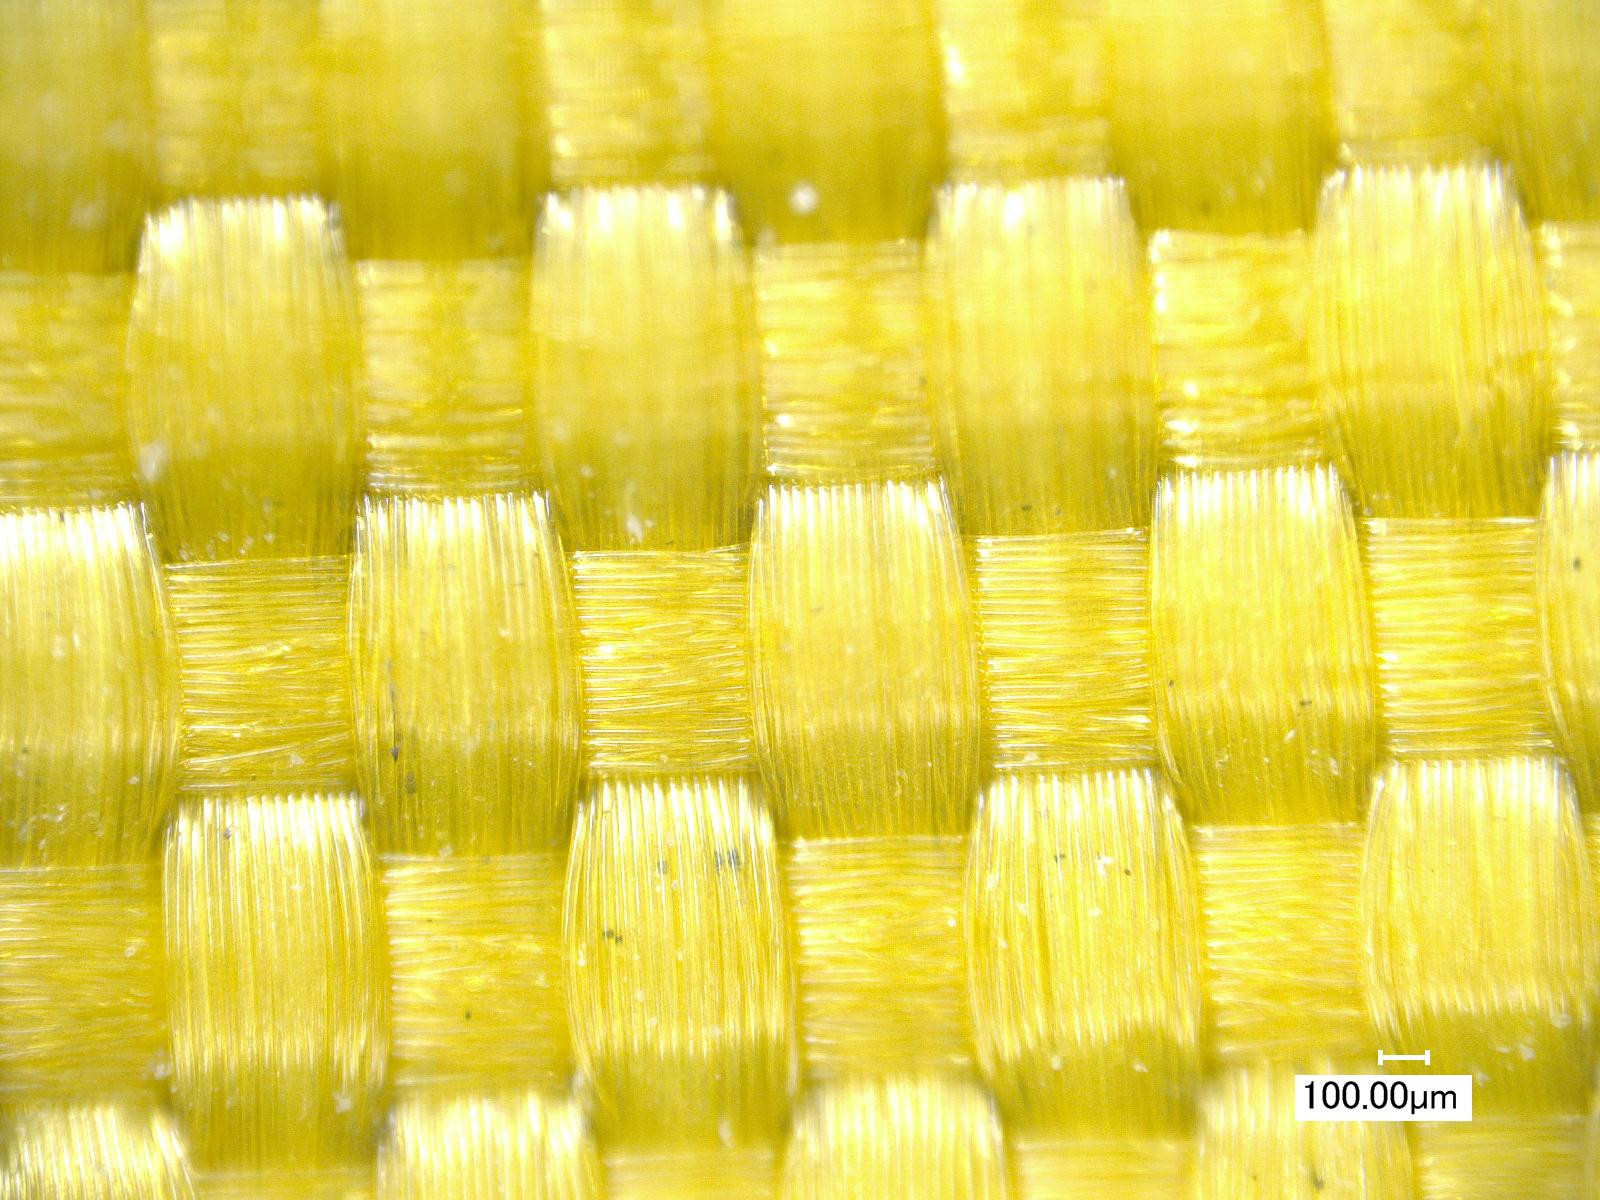
\includegraphics[keepaspectratio, width=0.8\linewidth]{figures/中心/カーリングパッド10-15低倍率.jpg}
            \caption{低倍率(100倍)}
            \label{fig:label}
        \end{minipage}
        \begin{minipage}[htbp]{0.45\linewidth}
            \centering
            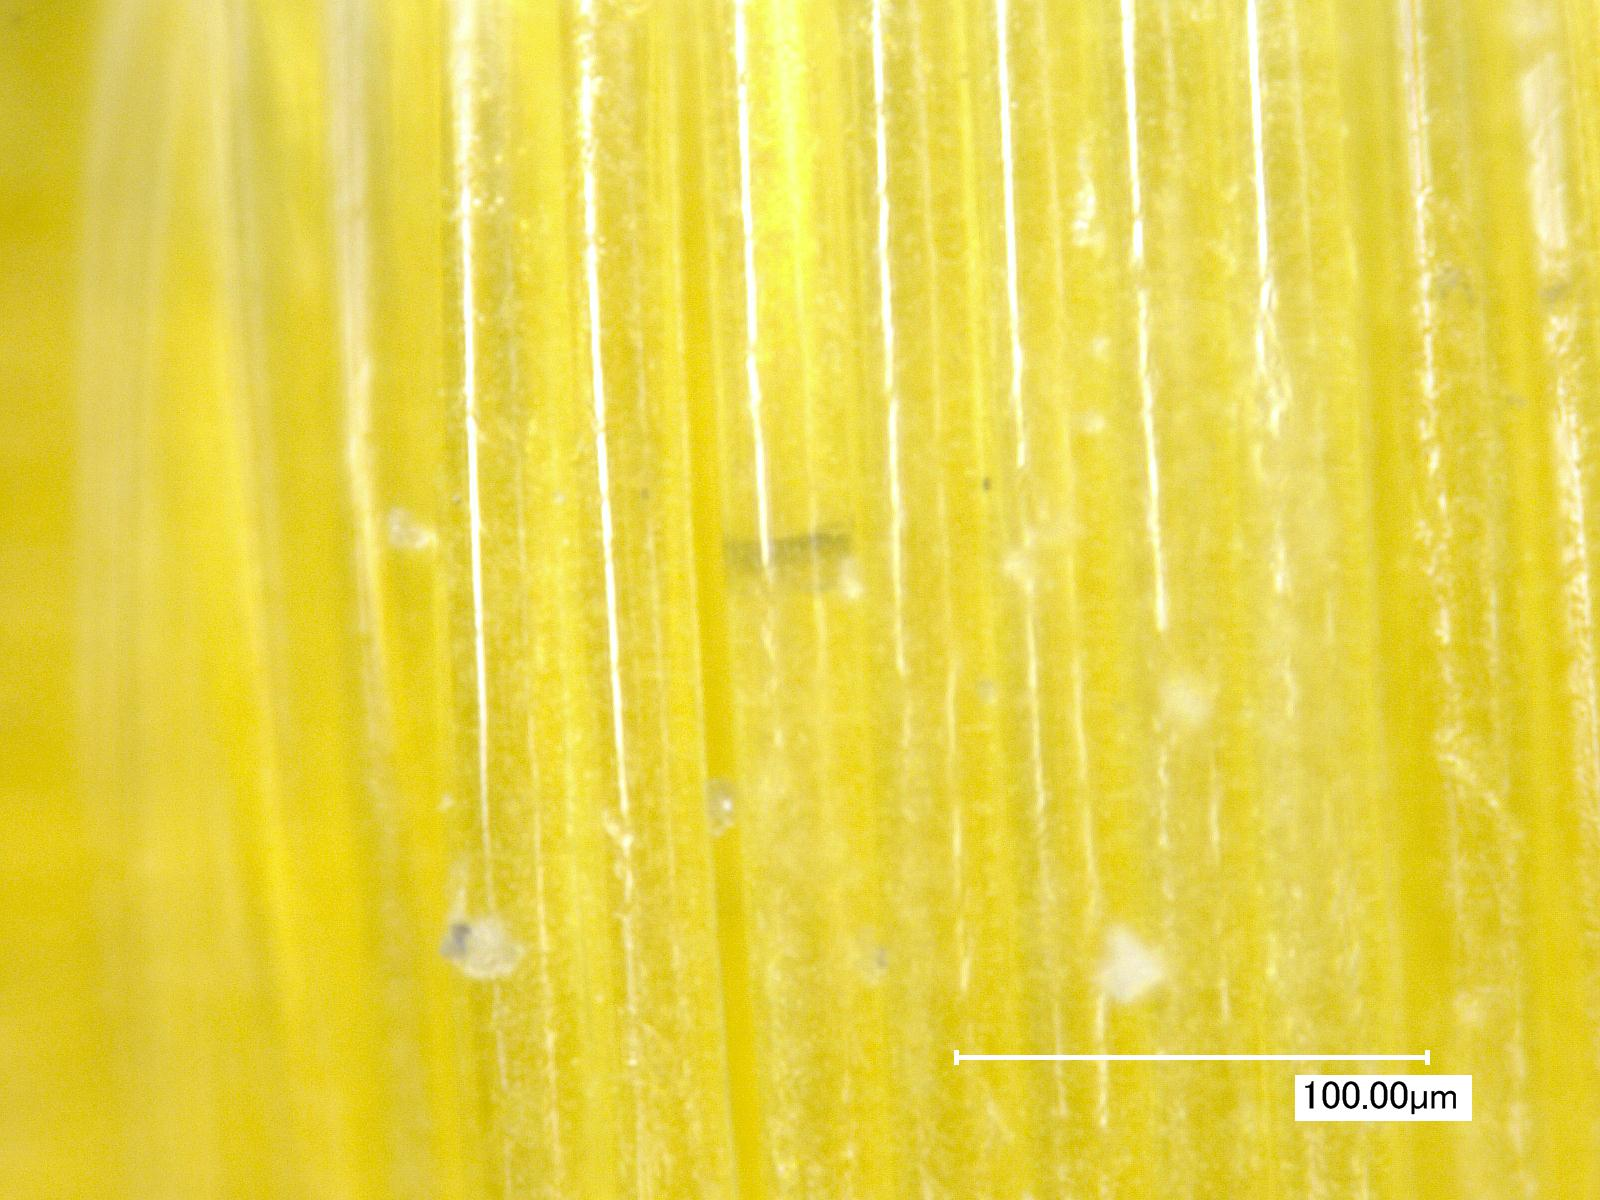
\includegraphics[keepaspectratio, width=0.8\linewidth]{figures/中心/カーリングパッド10-15.jpg}
            \caption{高倍率(1000倍)}
            \label{fig:label}
        \end{minipage}
    \end{figure}
    \item 長時間使用
    \begin{figure}[H]
        \centering
        \begin{minipage}[htbp]{0.45\linewidth}
            \centering
            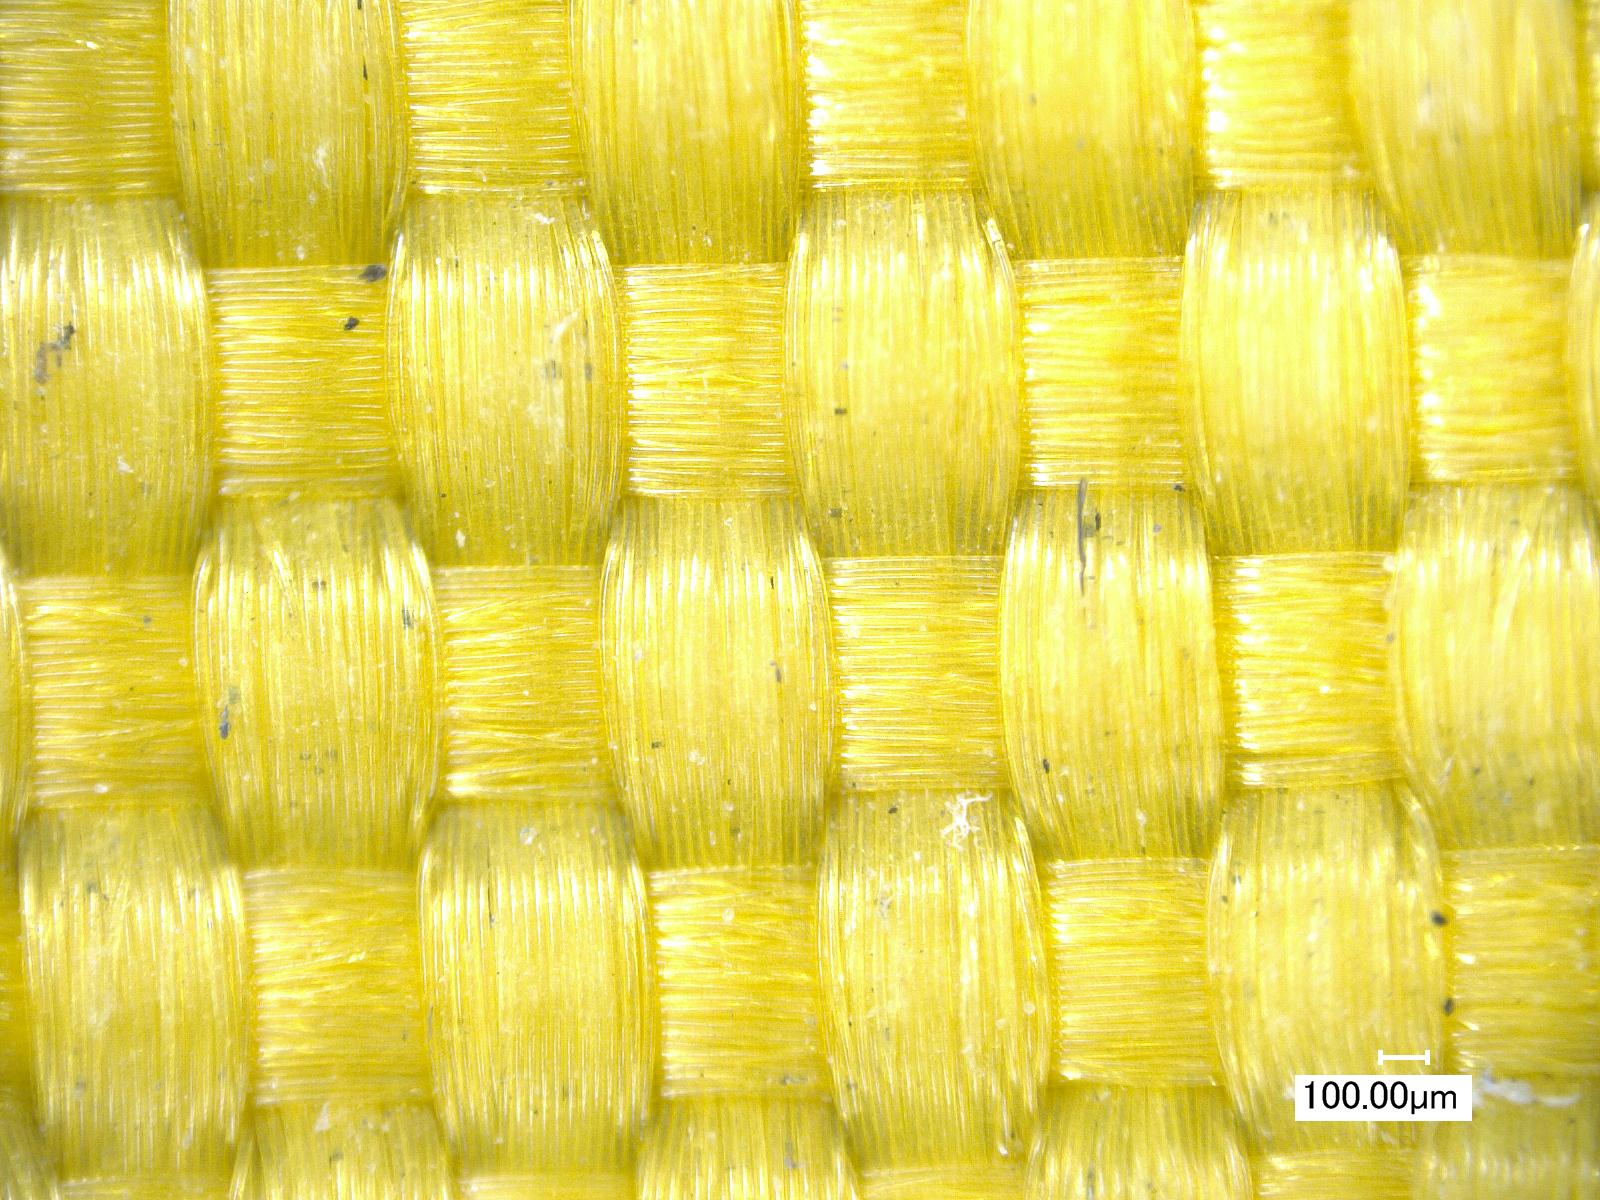
\includegraphics[keepaspectratio, width=0.8\linewidth]{figures/中心/カーリングパッド長期低倍率.jpg}
            \caption{低倍率(100倍)}
            \label{fig:label}
        \end{minipage}
        \begin{minipage}[htbp]{0.45\linewidth}
            \centering
            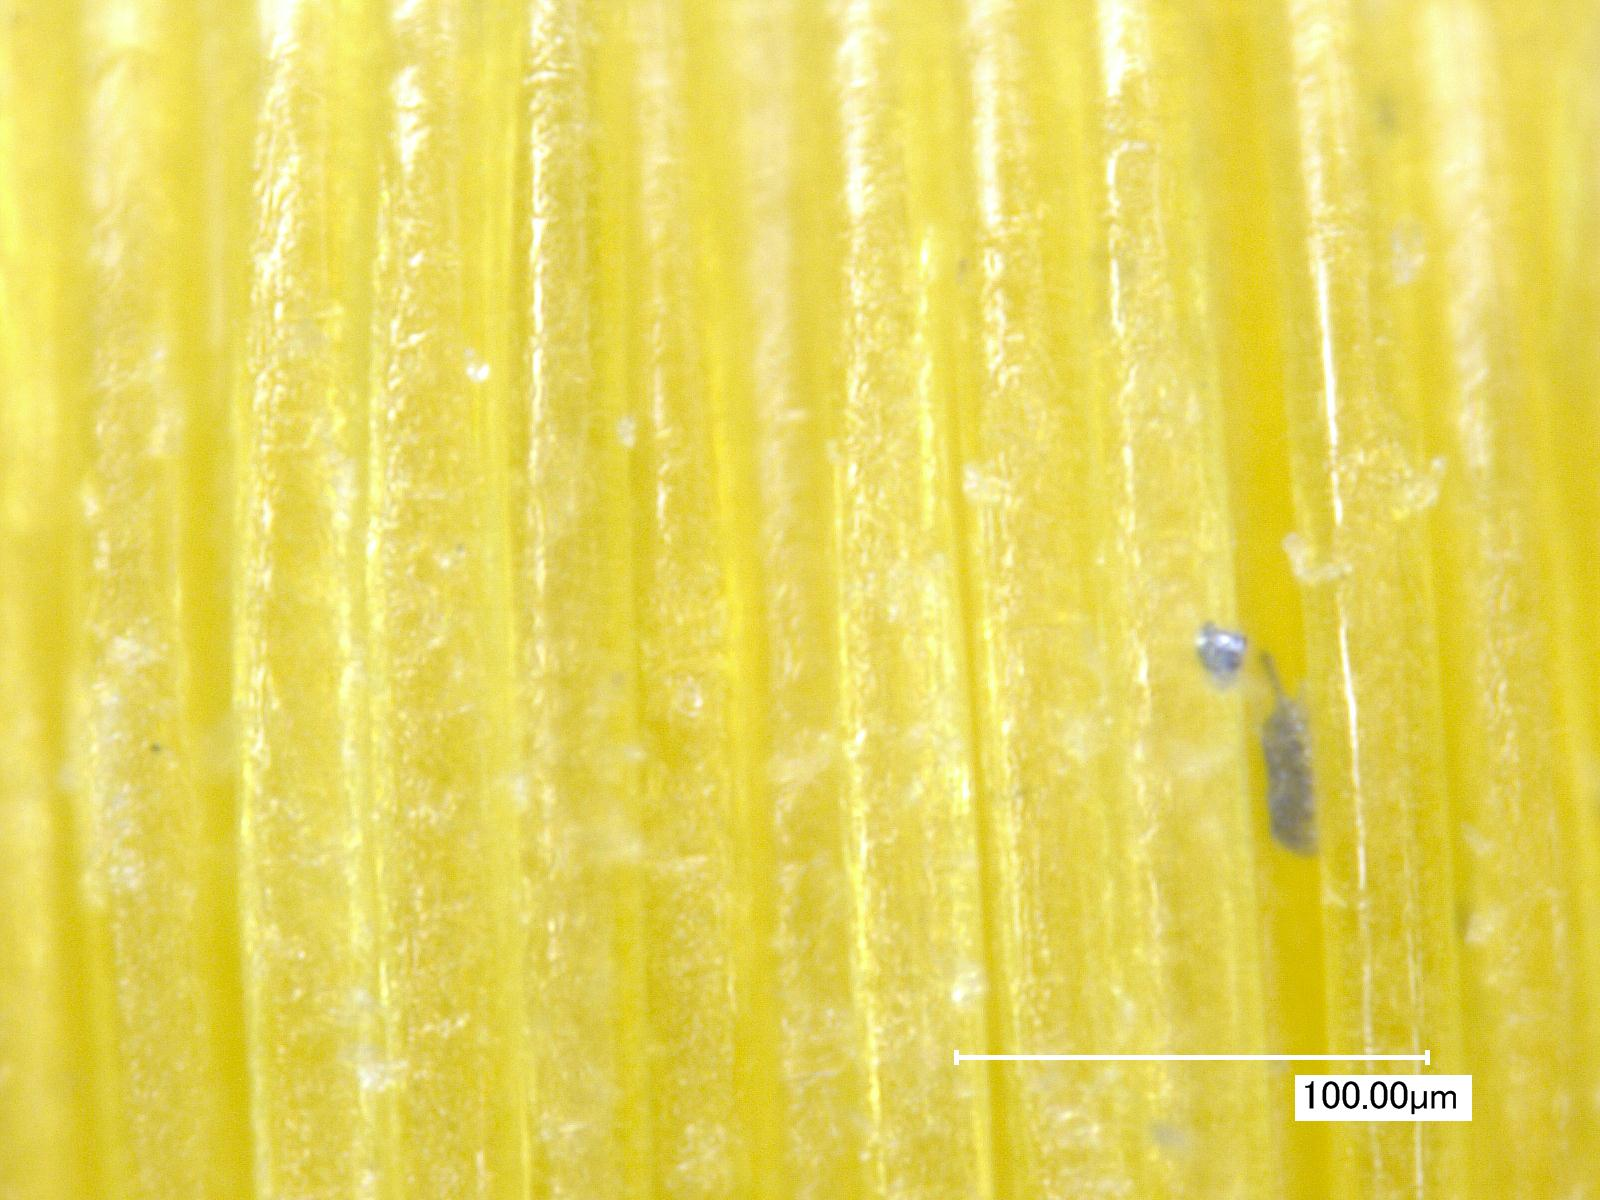
\includegraphics[keepaspectratio, width=0.8\linewidth]{figures/中心/カーリングパッド長期.jpg}
            \caption{高倍率(1000倍)}
            \label{fig:label}
        \end{minipage}
    \end{figure}
\end{itemize}

カーリングブラシパッドの中心の部分は長期間使用したものでも,未使用のもののように繊維が隙間なく並んでいた.
中心部分の表面には使用時間によって差はないことがわかった.

\end{document}